%%%%%%%%%%%%%%%%%%%%%%%%%%%%%%%%%%%%%%%%%%%%%%%%%%%%%%%%%%%%%%%%%%%%%%%%%%%%%%%%
%% Capitulo
%%%%%%%%%%%%%%%%%%%%%%%%%%%%%%%%%%%%%%%%%%%%%%%%%%%%%%%%%%%%%%%%%%%%%%%%%%%%%%%%
\chapterimage{chapter_head_carnaval2.pdf} % Chapter heading image

\chapter{Historia da música do samba}\index{Música do samba}


\begin{tcbinformation}{Samba}
\index{Samba}
\label{ref:samba} 
No Brasil, a palavra samba  é usada como designação de uma dança popular  
e música  em \hyperref[subsec:compassobinario]{\textbf{compasso binário}} (geralmente 2/4), 
de ritmo sincopado e \hyperref[sec:Andamento]{\textbf{andamento}} 
variado \cite[pp. 290]{dourado2004dicionario} \cite[pp. 684]{marcondes1977enciclopediav2};
ambos com uma forte influencia da cultura africana \cite[pp. 290]{dourado2004dicionario};
representando estas, desde inícios do século XX, 
uma expressão cultural, urbana e popular no Brasil \cite[pp. 684]{marcondes1977enciclopediav2} \cite[pp. 290]{dourado2004dicionario}. 
%a qual ao longo dos anos tem gerado uma grande variedade de subgêneros de dança e de música.
\end{tcbinformation}

~

\noindent 
\begin{minipage}{\textwidth}
\begin{wrapfigure}{r}{0.38\textwidth}
    \centering
    \vspace{-13pt}
    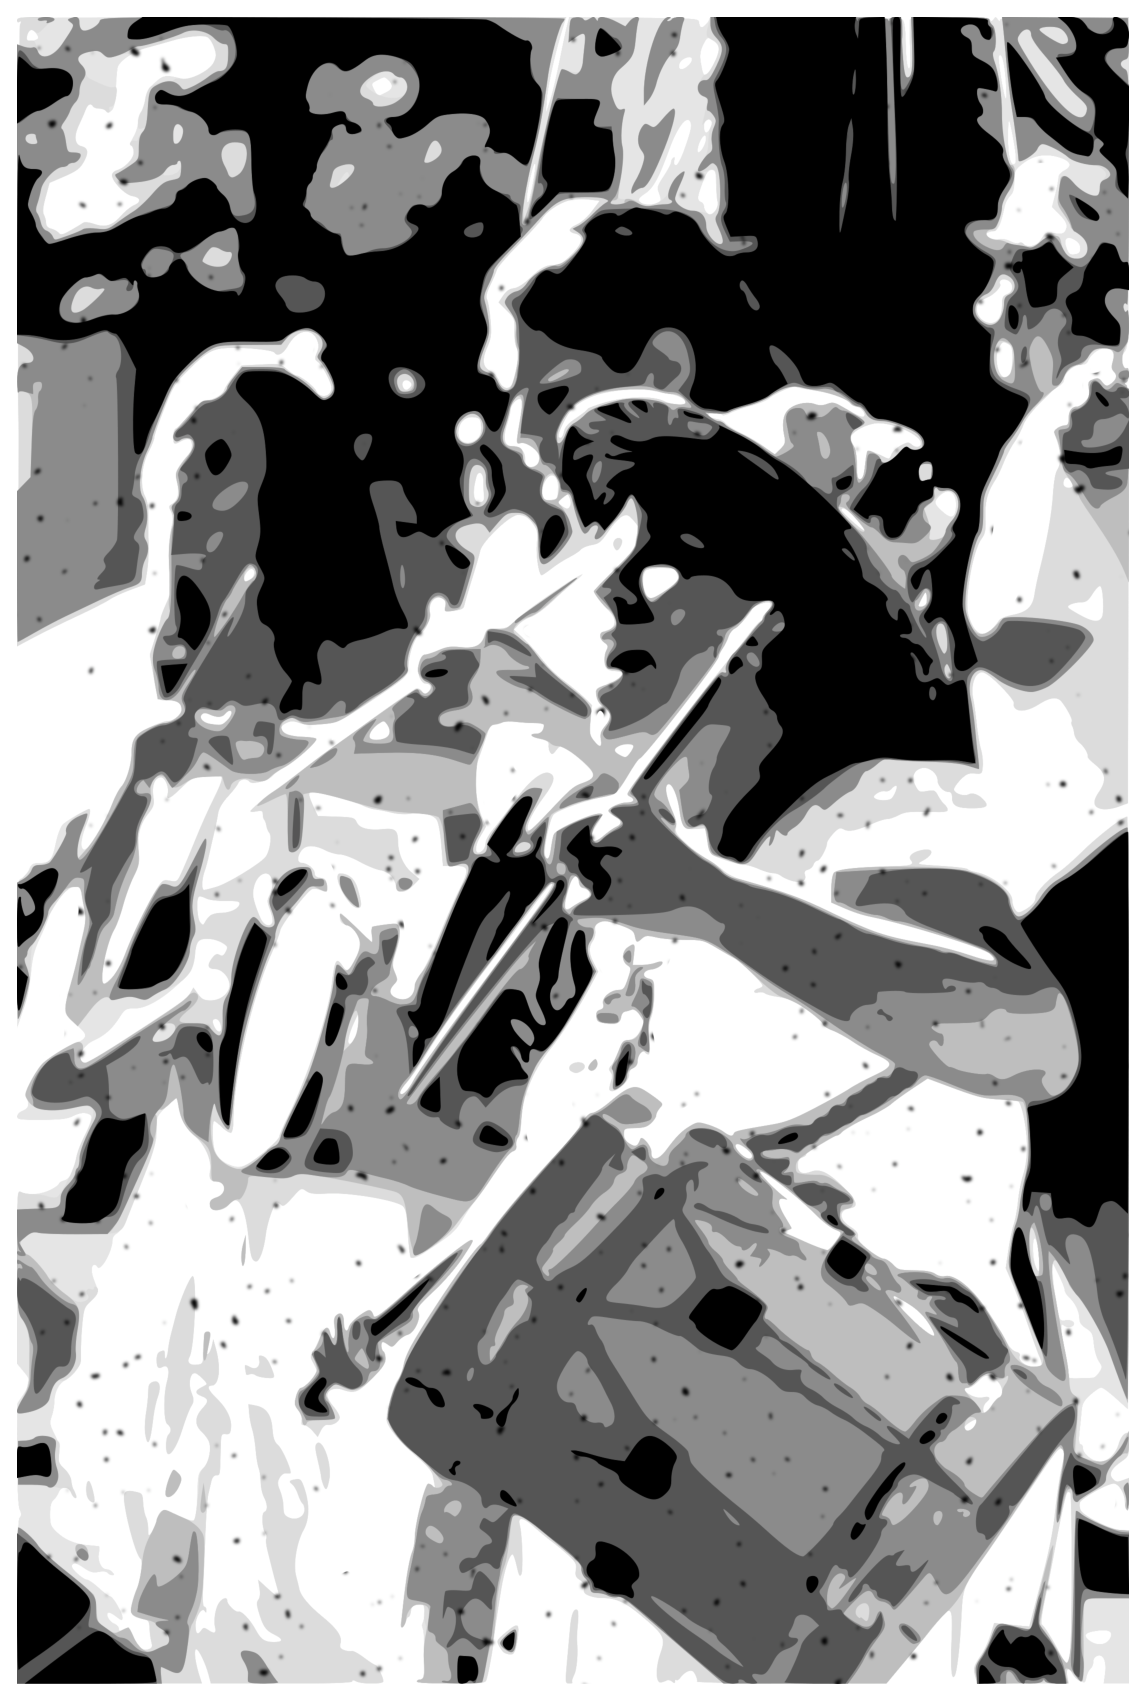
\includegraphics[width=0.34\textwidth]{chapters/cap-historia-musicasamba/DSC_0044-4-efeitoimagem-envelhecer.eps}
\end{wrapfigure}
\hspace{0.75cm} O samba é uns dos gêneros musicais mais conhecidos no Brasil do século XXI;
outros gêneros que tem muita popularidade são o ``forró'' e o ``sertanejo'', porém
%entre estes gêneros mais populares, temos por exemplo, ao ``forró'' e ao ``Sertanejo''; sendo que 
o samba tem se distinguido entre eles
como a principal expressão popular da música brasileira \cite[pp. 47]{diniz2008almanaque}.

A popularização, o reconhecimento comercial e a representatividade cultural no consciente coletivo do povo brasileiro
não sempre estiverem alinhados com o samba, 
sendo que esta conjunção teve seu origem a inícios do seculo XX, 
com o inicio das gravações comerciais em disco, 
momento no qual o samba teve uma grande popularização comercial.
%provocando a consequente popularização comercial do gênero.

Nas seguintes seções veremos um pouco das origens da música do samba e como
esta ficou popular no mundo discográfico. 
Adicionalmente serão descritos alguns dos subgêneros que o samba tem gerado.
\end{minipage}

%%%%%%%%%%%%%%%%%%%%%%%%%%%%%%%%%%%%%%%%%%%%%%%%%%%%%%%%%%%%%%%%%%%%%%%%%%%%%%%%
%%%%%%%%%%%%%%%%%%%%%%%%%%%%%%%%%%%%%%%%%%%%%%%%%%%%%%%%%%%%%%%%%%%%%%%%%%%%%%%%
\section{Pelo telefone}

 As reuniões na casa da Tia Ciata foram o cenário da criação do samba-maxixe ``Pelo telefone'',
 composto, em 1916, 
por Ernesto dos Santos (Donga) e Mauro de almeida 
(Peru dos Pés Frios) \cite[pp. 34]{diniz2006almanaque} \cite[pp. 49]{diniz2008almanaque} 
\cite{musicapelotelefone} \cite[pp. 28]{diniz2003almanaque}.

%%%%%%%%%%%%%%%%%%%%%%%%%%%%%%%%%%%%%%%%%%%%%%%%%%%%%%%%%%%%%%%%%%%%%%%%%%%%%%%%
\subsection{Cronologia de: Pelo telefone}
Dados da música \textbf{Pelo telefone}:
\index{Pelo telefone}
\begin{itemize}
\item 1916, novembro 6, é presentada uma petição de registro no
Departamento de Direitos Autorais, da Biblioteca Nacional, 
do Rio de Janeiro (RJ), 
por   Ernesto dos Santos  para o samba carnavalesco \textbf{Pelo telefone} \cite[pp. 599]{marcondes1977enciclopediav2}.
\item 1916, novembro 16, Ernesto dos Santos, 
anexa à petição um atestado que afirma que 
o samba carnavalesco \textbf{Pelo telefone}, 
foi executado em público pela primeira vez no
Cine-Teatro Velho o dia 25 de outubro de 1916,
este atestado foi subscrito por M.P. Cabrita e Julio Suckow \cite[pp. 599]{marcondes1977enciclopediav2}.
\item 1916, novembro 27, o registro foi efetivado com o número 3.295 \cite[pp. 599]{marcondes1977enciclopediav2}.
\item 1916, dezembro 16, a partitura manuscrita para piano, feita por Pixinguinha, 
estava dedicada a Mauro de Almeida e Norberto Amaral (Morcego) é
publicada no Instituto de Artes Gráficas, do Rio de Janeiro \cite[pp. 599]{marcondes1977enciclopediav2} \cite[pp 1]{revistausp1}.
\item Carnaval de 1917, a música foi sucesso   \cite[pp. 599]{marcondes1977enciclopediav2}  \cite[pp. 35]{diniz2006almanaque}, 

\item 1917, É realizada a primeira gravação de  \textbf{Pelo telefone}, feita pela Banda Ondeon (121.313-B), 
onde consta como autor unicamente Donga, 
sendo esta uma gravação instrumental \cite{musicapelotelefone} \cite[pp. 599]{marcondes1977enciclopediav2},
e  fabricada especialmente para a Casa Edison, pela fabrica Ondeon, com número de patente 3465.
\item 1917, É realizada a segunda gravação, na qual os versos de \textbf{Pelo telefone} seriam conhecidos pelo público;
foram encargados da interpretação, ``Bahiano\footnote{Está 
escrito Bahiano na capa do disco, porém muitas referencias bibliográficas,
escrevem Baiano.} e côro'' (121.322-A), acompanhado somente de violão e cavaquinho. 
Esta gravação é fabricada especialmente para a Casa Edison, pela fabrica Ondeon, com número de patente 3465,  
e constam como autores Donga e Mauro de Almeida 
(música e letra respetivamente) \cite[pp. 599]{marcondes1977enciclopediav2} 
\cite[pp. 35]{diniz2006almanaque}  \cite{musicapelotelefone}.
\end{itemize}

%%%%%%%%%%%%%%%%%%%%%%%%%%%%%%%%%%%%%%%%%%%%%%%%%%%%%%%%%%%%%%%%%%%%%%%%%%%%%%%%
\subsection{Autoria de: Pelo telefone}

A autoria de ``Pelo telefone'' é questionada por compositores contemporâneos de Donga, que alegam que
ele modificou e apropriou-se de uma criação coletiva e anônima, 
de tradição oral cantada por todos na casa da Tia Ciata \cite{musicapelotelefone} \cite[pp. 35]{diniz2006almanaque} \cite[pp. 49]{diniz2008almanaque};
assim, o dia 4 de Fevereiro de 1917, no ``Jornal do Brasil'' (RJ), Tia Ciata, Sinhô e outros,
protestaram a usurpação da autoria, parodiando à versão gravada, como é visto a seguir \cite[pp. 17]{TiaCiataVsDonga} \cite[pp. 118-119]{sandroni2001feitico}:
\begin{citando}%%
\begin{center}
1ra PARTE\\
Pelo telefone a minha boa gente\\
Mandou-me avisar!...\\
Que meu bom arranjo era oferecido\\
Para se cantar!...\\
~\\
2da PARTE\\
Ai! Ai! Ai!... leve a mão\\
A' consciencia!...\\
Meu bem,\\
Ai! Ai! Ai!... porque\\
Tanta presença!...\\
Meu bem!\\
~\\
1ra PARTE\\
O que cara dura de dizer nas rodas\\
Que este arranjo é teu?...\\
É do bom Hilario e da velha Ciatta\\
Que o Sinhô escreveu!...\\
~\\
3ra PARTE\\
Tomara que tu apanhes,\\
Para não tornar a fazer isso,\\
Escrever o que é dos outros,\\
Sem olhar o compromisso.
\end{center}
\end{citando}%%

Por outro lado, durante muito tempo ``Pelo telefone'' foi considerado o primeiro samba gravado;
porém, segundo Flávio Silva  já existiam outros discos anteriormente com a etiqueta samba,
inclusive pela Casa Edison, que gravou ``pelo telefone''  \cite[pp. 96]{hertzman2013making} \cite[pp. 118]{sandroni2001feitico}.

%%%%%%%%%%%%%%%%%%%%%%%%%%%%%%%%%%%%%%%%%%%%%%%%%%%%%%%%%%%%%%%%%%%%%%%%%%%%%%%%
\subsection{Relevância de: Pelo telefone}
Apesar de todos estes problemas, há uma contribuição de ``Pelo telefone'' à música, 
esta foi a indicação do gênero ``samba'' no selo do disco junto com o registro na Biblioteca Nacional,
que abriu o caminho para a difusão comercial e urbanização do gênero samba,
 e seu consequente prestigio \cite{musicapelotelefone} \cite[pp. 49]{diniz2008almanaque};
como corrobora Flávio Silva, que no seu levantamento bibliográfico deteta que, no carnaval, o termo
samba aparece na prensa  de Rio de Janeiro \cite[pp. 118]{sandroni2001feitico}, 
\begin{itemize}
\item 3 vezes em 1916, 
\item 22 vezes em 1917 e
\item 37 vezes em 1918.
\end{itemize}


%%%%%%%%%%%%%%%%%%%%%%%%%%%%%%%%%%%%%%%%%%%%%%%%%%%%%%%%%%%%%%%%%%%%%%%%%%%%%%%%
%%%%%%%%%%%%%%%%%%%%%%%%%%%%%%%%%%%%%%%%%%%%%%%%%%%%%%%%%%%%%%%%%%%%%%%%%%%%%%%%
\section{Qual é a família do samba (música)?}
\label{sec:FamiliaSamba}
\begin{tcbinformation}{Batucada (música)}
\index{Batucada}
\index{Música do samba!Batucada}
É a denominação dada ao ritmo do 
\hyperref[ref:batuquedanca]{\textbf{batuque}}\footnote{Para 
mais informação sobre o batuque ir a páginas \pageref{ref:batuquedanca1800} e \pageref{ref:batuquedanca}.} 
e é também usado como sinônimo deste \cite[pp. 89]{marcondes1977enciclopedia}.
\end{tcbinformation}
Existem muitos subgêneros em que o samba é tocado e cantado, alguns tiveram vida efêmera,
e outros perduraram no tempo, a continuação serão listados alguns subgêneros do samba,
incluindo o Maxixe, gênero musical que influenciou o samba.
% leer https://bndigital.bn.gov.br/exposicoes/ai-ai-ai-cem-anos-o-samba-faz/ritmos-que-influenciaram-o-samba/


%% MARACATU

%%%%%%%%%%%%%%%%%%%%%%%%%%%%%%%%%%%%%%%%%%%%%%%%%%%%%%%%%%%%%%%%%%%%%%%%%%%%%%%%
\subsection{Bossa nova} 
\index{Música do samba!Bossa nova}
\index{Música do samba!Samba-bossa}
Também chamado \textbf{samba-bossa}, este gênero pode ser entendido como um samba-choro modernizado \cite[pp. 63]{reinato2010musica}.
A bossa nova surgiu  na década de 1950 \cite[pp. 130]{perna2002samba},
apos a segunda gerra mundial pela influencia da cultura norte-americana, motivada 
pela política desenvolvimentista do presidente do Brasil, Juscelino Kubitschek (1956 - 1961) \cite[pp. 15]{de2003tem}.
Esta variante do samba é caraterizada por uma sofisticada harmonia e um modo diferente de dividir o fraseado, 
agregando influencias do impressionismo erudito do jazz  \cite[pp. 130]{perna2002samba} \cite[pp. 15]{de2003tem}. 

O inicio da bossa nova, e sua popularização, 
marcou um período de dificuldade para o choro e seus instrumentistas,
pelo desinteresse  do choro ao ser considerada coisa de velho, quadrada, nacionalista, de aposentado e suburbano \cite{rizzi2016musica}.

A bossa nova foi inaugurada usando composições e interpretações de, Antônio Carlos Jobim (Tom Jobim) e Carlos Lyra,
a poesia de Vinícius de Moraes, e
a batida do violão de João Gilberto \cite[pp. 130]{perna2002samba}  \cite[pp. 15]{de2003tem}.
\begin{example} ~

\begin{itemize}
\item ``Chega de saudade'' (1958) de Vinícius de Moraes e Antônio Carlos Jobim \cite{castro2016chega} \cite{tomjobim}.
\item ``Garota de Ipanema'' (1962) de Vinícius de Moraes e Antônio Carlos Jobim \cite{tomjobim}.
\end{itemize}
\end{example}

%%%%%%%%%%%%%%%%%%%%%%%%%%%%%%%%%%%%%%%%%%%%%%%%%%%%%%%%%%%%%%%%%%%%%%%%%%%%%%%%
\subsection{Choro}\label{subsec:musicchoro}
\index{Música do samba!Choro}
Este é um gênero musical brasileiro, surgido na cidade de São Sebastião, Rio de Janeiro, por volta de 1870 \cite[pp. 14]{diniz2003almanaque} \cite[pp. 132]{perna2002samba} \cite[pp. 64]{reinato2010musica},
com espirito melancólico que mesclou o samba com  estilos europeus como schottisches, polcas,
valsas e outros gêneros em voga na época  \cite[pp. 64]{reinato2010musica} \cite[pp. 79]{dourado2004dicionario} \cite[pp. 132]{perna2002samba}.
O choro ou chorinho é uma composição livre, em ritmo binário, 
tradicionalmente composto em três seções com 16 \hyperref[sec:compaso]{\textbf{compassos}} cada uma \cite[pp. 64]{reinato2010musica}.
Para o ano de 1910 este já era um gênero consolidado \cite[pp. 12]{diniz2003almanaque}.

Entre os instrumentos mais populares que constituíram o choro na época da criação, 
estão o violão, o cavaquinho e a flauta transversal;
na década de 1930 foram incorporados, o pandeiro, o bandolim e a clarineta \cite[pp. 64]{reinato2010musica} \cite[pp. 79]{dourado2004dicionario} \cite[pp. 132]{perna2002samba};
todos estes instrumentos dão à música um aspecto sentimental melancólico e ``choroso'', e
é de ali que alguns autores apontam que surge o nome do estilo \cite[pp. 132]{perna2002samba};
porém, seguindo Batista Siqueira, 
o termo choro vem da fusão do verbo ``chorar'' e ``chorus'', coro em latim \cite[pp. 13]{diniz2003almanaque}.

O flautista, Joaquim Callado (Joaquim Antônio da Silva Callado 1848-1880) 
é conhecido como ``O pai do choro'';
este foi o autor de 66 melodias, e conseguiu conciliar: 
uma sólida formação musical com um grande poder de improvisação  \cite[pp. 15]{diniz2003almanaque} \cite[pp. 64]{reinato2010musica}.
Entre os grandes interpretes do gênero temos a:
Pixinguinha, Waldir Azevedo, Jacó do Bandolim, Dinho Sete Cordas, Altamiro Carillo \cite[pp. 79]{dourado2004dicionario}, etc.

\begin{example} ~

\begin{itemize}
\item ``Querida por todos'' (1869) de Joaquim Callado \cite[pp. 15]{diniz2003almanaque} \cite[pp. 1089]{marcondes1977enciclopediav2}.
\item ``Cruzes, minha prima'' (1875) de Joaquim Callado \cite[pp. 15]{diniz2003almanaque} \cite[pp. 951]{marcondes1977enciclopediav2}.
\item ``A flor amorosa'' (1880) de Joaquim Callado \cite[pp. 8]{livingston2005choro} \cite[pp. 15]{diniz2003almanaque}  \cite[pp. 985]{marcondes1977enciclopediav2}.
\item ``Tico-Tico no fubá'' (1917) de Zequinha de Abreu; sem letra, foi chamado na época ``Tico-Tico no farelo'' \cite[pp. 6]{marcondes1998enciclopedia} \cite[pp. 39,91]{diniz2003almanaque}.
\item ``Carinhoso'' (1927) Pixinguinha   \cite[pp. 133]{perna2002samba}.
\item ``Brasileirinho'' (1947) de Valdir Azevedo  \cite[pp. 133]{perna2002samba}.
\item ``Noites cariocas'' Jacob do Bandolim \cite{diniz2003almanaque}.
\item ``Doce de coco'' Jacob do Bandolim \cite{diniz2003almanaque}.
\item ``Vibrações'' Jacob do Bandolim \cite{diniz2003almanaque}.
\item ``Melodia celestial'' de Raul Barros \cite[pp. 130]{livingston2005choro}.
\end{itemize}
\end{example}

%%%%%%%%%%%%%%%%%%%%%%%%%%%%%%%%%%%%%%%%%%%%%%%%%%%%%%%%%%%%%%%%%%%%%%%%%%%%%%%%
\subsection{Marchinha} 
\label{subsec:marcha}
\index{Música do samba!Marchinha}
\index{Música do samba!Marcha}
Também chamado \textbf{marcha} \cite[pp. 448]{marcondes1977enciclopedia},
é um gênero de música popular, em \hyperref[subsec:compassobinario]{\textbf{compasso binário}} (2/4) de \hyperref[sec:Andamento]{\textbf{andamento}} vivo, 
está provem dos ranchos e cordões carnavalescos, a coreografia consiste num andar ritmado e em voltas. \cite[pp. 65]{reinato2010musica}.

A diferença entre a marcha-rancho e  a marchinha está no jeito cadenciado, 
melodioso e harmônico da primeira, em contrapartida ao estilo espevitado,
jocoso, cheio de sátiras e com letras de duplo sentido da segunda \cite[pp. 84,87]{diniz2008almanaque}.

A primeira marchinha carnavalesca, titulada ``Ô abre alas'', foi escrita em 1899 por Chiquinha Gonzaga \cite[pp. 84, 239]{diniz2008almanaque}.

\begin{example} ~

\begin{itemize}
\item ``Ô abre alas'' (1899) Chiquinha Gonzaga  \cite[pp. 84, 239]{diniz2008almanaque}.
\item ``Os calças-largas'' (1927) Lamartine Babo e Francisco Gonçalves de Oliveira,
interpretado por Frederico Rocha \cite[pp. 91]{diniz2008almanaque}.
\item ``O teu cabelo não nega'' (1932) de Lamartine Babo e dos Irmãos Valença, interpretado por Castro Barbosa \cite[pp. 99]{diniz2008almanaque}.
\item ``Balancê'' (1936) de Alberto Ribeiro e Braguinha interpretado por Carmen Miranda \cite[pp. 83]{diniz2008almanaque}.
\item ``Mamãe, eu quero'' (1937) de Vicente Paiva e Jararaca \cite[pp. 584]{marcondes1977enciclopediav2} \cite[pp. 93]{diniz2008almanaque}.
\item ``Cabeleira do Zezé'' (1964) de João Roberto Kelly e Roberto Faissal interpretado por Jorge Goulart \cite[pp. 117,118]{diniz2008almanaque}.
\item ``Pierrô apaixonado'' (1936) de Heitor dos prazeres e Noel Rosa \cite[pp. 1070]{marcondes1977enciclopediav2} \cite[pp. 53]{diniz2008almanaque}.
\end{itemize}
\end{example}

%%%%%%%%%%%%%%%%%%%%%%%%%%%%%%%%%%%%%%%%%%%%%%%%%%%%%%%%%%%%%%%%%%%%%%%%%%%%%%%%
\subsection{Marcha-rancho}
\index{Música do samba!Marcha-rancho}
Inicialmente chamado de \textbf{marcha de rancho} \cite[pp. 448]{marcondes1977enciclopedia}
é um gênero de musica popular, em \hyperref[subsec:compassobinario]{\textbf{compasso binário}} andante, 
está provem da musica produzida pelas chamadas orquestras dos ranchos e cordoes 
carnavalescos de fins da década de 1910 \cite[pp. 65]{reinato2010musica} \cite[pp. 448]{marcondes1977enciclopedia}.

A marcha-rancho tem um ritmo mais dolente que o das marchas (marchinhas)
e tem muito mais trabalho na parte melódica. 
Este gênero foi desenvolvido por autores reconhecidos, 
a finais da década de 1920;
onde podemos ver composições como a marcha rancho com coro ``moreninha'',
gravada no disco Ondeon n. 123.208, em 1927 \cite[pp. 448]{marcondes1977enciclopedia}.

\begin{example} ~

\begin{itemize}
\item ``Moreninha'' (1927) de Eduardo Souto \cite[pp. 448]{marcondes1977enciclopedia}
%\item ``Bem-te-vi'' (1933) de Lamartine Babo interpretado por Gastão Formenti \cite[pp. 916]{marcondes1977enciclopediav2} \cite[pp. 87]{diniz2008almanaque}.
\item ``As Pastorinhas'' (1938) de Carlos Alberto Ferreira Braga (Braguinha ou João de Barro) e Noel Rosa, 
inicialmente titulado ``Linda pequena''.
Apos modificação de nome, letra e música, 
foi regravado e interpretado por Sílvio Caldas \cite[pp. 1066]{marcondes1977enciclopediav2} \cite[pp. 87]{diniz2008almanaque}.
\item ``Marcha da quarta-feira de cinzas'' (1962) de Vinícius de Moraes e Carlos Lyra \cite[pp. 1021]{marcondes1977enciclopediav2} \cite[pp. 91]{diniz2008almanaque}.
\item ``A banda'' (1966) Chico Buarque interpretada por Nara Leão \cite[pp. 90]{diniz2008almanaque} \cite{partituraabanda1}.
\item ``Máscara negra'' (1967) José Flores de Jesus (Zè Kéti)  \cite[pp. 89]{diniz2008almanaque}.
\item ``Flor do sereno'' (2000)  \cite[pp. 88]{diniz2008almanaque}.

\end{itemize}
\end{example}

%%%%%%%%%%%%%%%%%%%%%%%%%%%%%%%%%%%%%%%%%%%%%%%%%%%%%%%%%%%%%%%%%%%%%%%%%%%%%%%%
\subsection{Maxixe}
\label{subsec:maxixe}
\index{Música do samba!Maxixe}
Também chamado \textbf{machiche}\footnote{Seguindo Batista Siqueira, 
o termo maxixe é uma corruptela de ``Macho, viche'', 
de ``sou macho, virgem'', e por conseguinte devia ser escrito machiche \cite[pp. 198]{dourado2004dicionario}.}.
Na época se acreditava que o nome seria em aluição de uma fruta que brotava junto ao capim dos piores recantos cariocas,
como a zona de baixo meretricio do Mangue do Rio de Janeiro \cite[pp. 198]{dourado2004dicionario}.
O maxixe designou durante certo tempo à música brasileira característica da cidade, 
ate que cedeu seu lugar ao samba \cite[pp. 4]{musicasambavariasdef1}.

O maxixe é composto de ritmos sincopados, com ascendência de ritmos africanos \cite[pp. 198]{dourado2004dicionario}.
Esta é uma música afro-brasileira \cite[pp. 4]{musicasambavariasdef1} 
que foi criada para dar contexto ao  maxixe (dança), que já existia e era dançado em vários gêneros musicais da época.
O maxixe (música) só foi reconhecida pelas casas musicais como um gênero musical no final do seculo XIX \cite[pp. 465]{marcondes1977enciclopedia}. 
Este gênero resultou da fusão do ritmo do tango e a havanera, 
do \hyperref[sec:Andamento]{\textbf{andamento}} da polca e 
a sincopa de músicas com ascendência africana como o lundu  \cite[pp. 29]{efege1974maxixe}  \cite[pp. 465]{marcondes1977enciclopedia}. 

O primeiro maxixe impresso com a respectiva menção de gênero, é ``Ora bolas!'' de Juca Storoni em 1897,
sendo este nome um pseudônimo, o que da uma indicação do estigma da época aos compositores deste gênero \cite[pp. 80]{sandroni2001feitico} \cite[pp. 108]{efege1974maxixe}.

\begin{example} ~

\begin{itemize}
\item ``Ora, bolas!'' (1897) de Juca Storoni \cite[pp. 108]{efege1974maxixe}.
\item ``Gaucho (Corta-Jaca)'' (1897) de Chiquinha Gonzaga \cite{reportagemtvmaxixe} \cite[pp. 30]{efege1974maxixe}.
\item ``Maxixe da Guarda Velha'' (1899) com letra de Arthur Azevedo, 
e música do compositor paulista Nicolino Milano  \cite{reportagemtvmaxixe}. 
\item ``Maxixe Aristocrático'' (1904) de José Nunes \cite{REIS2003}.
\item ``Vem cá, mulata'' (1906) de José do Patrocínio Filho, Chicot e Thoreau \cite{REIS2003}.
\item ``Forrobodó'' (1912) de Chiquinha Gonzaga \cite{REIS2003} \cite{reportagemtvmaxixe}.
\item ``Jocotó'' Roque V. Vieira \cite{reportagemtvmaxixe}.
\end{itemize}
\end{example}

%%%%%%%%%%%%%%%%%%%%%%%%%%%%%%%%%%%%%%%%%%%%%%%%%%%%%%%%%%%%%%%%%%%%%%%%%%%%%%%%
\subsection{Pagode}
\index{Música do samba!Pagode}
Também chamado \textbf{samba de fundo do quintal}  \cite[pp. 130]{perna2002samba}.
No Rio de Janeiro, pagodes são locais de reunião informal, quintais cobertos, e outros,
que davam espaço a um pequeno baile pre carnavalesco, 
rodas de samba ou de partido-alto, criadas geralmente por músicos amadores \cite[pp. 130]{perna2002samba} \cite[pp. 241]{dourado2004dicionario} \cite[pp. 241]{dourado2004dicionario}.
Assim, nestos locais se cantavam ritmos populares principalmente samba,
geralmente acompanhados de percussão, cavaquinho e violão, 
de modo que este  estilo de fazer música passou a ser chamado de pagode \cite[pp. 63]{reinato2010musica}  \cite[pp. 130]{perna2002samba}.

Ao final da década de 1960 saíram os primeiros sambistas classificados como pagodeiros,
porém a origem do pagode seria anterior a este período \cite{sedano2018bezerra}.
Os sambistas de Rio de Janeiro desde os tempos da Tia Ciata, 
falavam pagode para designar ao samba de forma carinhosa; 
assim, samba e pagode era entendido como uma coisa só, uma festa, 
onde as pessoas se reuniam, cantavam, dançavam, comiam e ate paqueravam \cite[pp. 209]{diniz2006almanaque}.

O bloco carnavalesco ``Cacique de Ramos'' teria sido o centro irradiador do pagode no final da década de 1960,
sendo este o promotor do ressurgimento do gênero no cenário musical brasileiro \cite{sedano2018bezerra},
com seus reuniões  para um pagode todas as quartas feiras  \cite[pp. 210]{diniz2006almanaque}.

Apos o ano 1970 a industria da música no Brasil sofreu uma crise que afetou a produção musical, 
incluindo ao pagode;
porém a partir do ano de 1981, o mercado musical retomou seu interesse pelo pagode \cite{sedano2018bezerra}.
com nomes como: Zeca Pagodinho, Agepê, Almir Guineto, Alicione, 
Jorge Aragão e Jovelina Pérola Negra \cite[pp. 130]{perna2002samba} \cite{sedano2018bezerra};
sendo, ``fundo de quintal'' (1980), o primeiro ``grupo'' de pagode \cite[pp. 130]{perna2002samba} \cite{fundodequintal}.

Em 1985, a gravadora RGE lançou o LP chamado  ``Raça brasileira'', 
sendo este projeto mas que uma coletânea, um marco fonográfico e cultural,
do fenômeno conhecido como pagode. Este projeto contou com a colaboração de artistas como:
Zeca Pagodinho, 
Jovelina Pérola Negra, 
Eliane Machado,
Pedrinho da Flor e
Mauro Diniz \cite[pp. 211]{diniz2006almanaque}.

Estes artistas antes identificados como pagodeiros, mudaram seu status em 1990, 
 quando apareceram grupos de ``pagode romântico'', 
de modo que os pagodeiros da antiga passaram a chamar-se como ``sambista de raiz''  \cite{sedano2018bezerra}. 

\begin{example} LP ``Raça brasileira'' lançado em 1985:

\begin{itemize}
\item ``Raça Brasileira'' interpretado por Elaine Machado.
\item ``Leilão'' interpretado por Zeca Pagodinho.
\item ``Que Maravilha (Maravilhas do Amor)'' interpretado por Pedrinho Da Flor.
\item ``Feirinha da Pavuna (Confusão de Legumes)'' interpretado por Jovelina Pérola Negra.
\item ``Mal de Amor''  interpretado por  Mauro Diniz.
\item ``Pot-Pourri Santa Paciência/Bamba de Berço'' interpretado por Zeca Pagodinho, Mauro Diniz.
\item ``Garrafeiro'' interpretado por Zeca Pagodinho.
\item ``Pingueira'' interpretado por Elaine Machado.
\item ``Ingrata Paixão'' interpretado por Mauro Diniz.
\item ``Pomba-Rolou'' interpretado por  Jovelina Pérola Negra.
\item ``A Vaca'' interpretado por Zeca Pagodinho.
\item ``Pot-Pourri Pedra No Caminho/Bagaço da Laranja'' interpretado por Zeca Pagodinho, Jovelina Pérola Negra e Pedrinho Da Flor.
\end{itemize}
\end{example}

%%%%%%%%%%%%%%%%%%%%%%%%%%%%%%%%%%%%%%%%%%%%%%%%%%%%%%%%%%%%%%%%%%%%%%%%%%%%%%%%
\subsection{Sambalanço}
\label{ref:sambalanco}
\index{Música do samba!Samba balanço}
\index{Música do samba!Sambalanço}
O sambalanço e um gênero musical,
que se encontra num ponto intermédio entre o samba tradicional (de morro e batucada)
e a bossa nova (samba estilizado), e surgiu na década de 1950 \cite[pp. 119]{diniz2008almanaque}.
Onde vários compositores, interpretes e músicos, 
transformaram a bossa nova dando-lhe maior impacto rítmico e uma nova estrutura instrumental,
numa amalgama que agora conhecemos como sambalanço, \textbf{balanço} ou \textbf{samba de balanço} \cite{de2017sambalanco}.

Carlos Lyra procurando uma denominação para sua música, 
pois achava que esta já não tinha direito de ser chamado de bossa nova,
achou no termo sambalanço, mescla de samba e balanço, a designação mais apropriada para esta \cite{castro2011bossa};
este nome foi inscrito por ele no registro de marcas e patentes \cite[pp. 127]{vianna1999bezerra} \cite{castro2011bossa}.


Carlos Lyra lança em 1961  seu segundo LP \cite[pp. 142]{lyrasongbook}  \cite{castro2011bossa}, 
tendo nesta ocasião a colaboração de Vinícius de Moraes,
este último, escreve na contra portada do LP um comentário sobre Lyra e o sambalanço,
indicando que a música de Carlos, pertence à corrente mais nacionalista da bossa nova,
pelo qual este sentiu a necessidade de dar um nome próprio a sua obra, 
chamando-o de sambalanço, 
porém Vinícius questiona a necessidade do nome e reafirma que a expressão 
 bossa nova tem a amplitude necessária para cobrir sem espirito de divisão esta música \cite{castro2011bossa}.

Segundo Orlandivo o sambalanço é ``uma música que tira você, nem que fique em pé dançando sozinho ali'';
sendo este estilo muito diferente da bossa nova, pois nesta última por mais que você queira dançar, fica difícil;
a bossa nova é uma música para escutar sentado \cite{de2017sambalanco}.
\begin{example} ~

\begin{itemize}
\item ``Era Bom'' (1960) de Hianto de Almeida e Macedo Neto  \cite[pp. 123]{de2003tem}.
\item ``Só amor'' (1961) de Vinícius De Moraes no segundo LP de Carlos Lyra \cite[pp. 142]{lyrasongbook}  
\item ``Tem que balançar'' (1961) de Carlos Imperial  \cite{de2017sambalanco}.
\item ``Gamação'' (1962) de João Roberto Kelly \cite[pp. 122]{de2003tem}.
\item ``Só vou de balanço'' (1963) de João Roberto Kelly \cite{de2017sambalanco}.
\item ``Na Roda do Samba'' (1964) de Orlandivo e Helton Menezes \cite{de2017sambalanco} \cite[pp. 122]{de2003tem}.
\item ``Toque Balanço, Moço!'' (1965) de Roberto Carlos e Erasmo Carlos \cite{de2017sambalanco} \cite[pp. 123]{de2003tem}.
\end{itemize}
\end{example}

\textbf{Sambalanço da década de 1990:} Também chamado \textbf{pagode paulista}  \cite[pp. 130]{perna2002samba}.
Durante os anos de 1994 e 1995, 
foi usado pela mídia o termo sambalanço, para designar a um certo tipo de música, 
bem diferente estilisticamente ao de 1950;
sendo este novo sambalanço um pagode relacionado a uma identidade nacional,
com uma atenção maior da mídia a este novo gênero \cite[pp. 127]{vianna1999bezerra}, 
e influenciada pela ``soul music'' norte-americana e a música romântica dos grupos sertanejos da época  \cite[pp. 130-131]{perna2002samba}.
Dentro desse novo sambalanço podemos ver grupos originários de São Paulo como, Raça negra e o Grupo Raça;
e ao grupo originário de Minas Gerais: Só pra contrariar \cite[pp. 130]{perna2002samba} \cite[pp. 128]{vianna1999bezerra}.
Outros nomes relativos a este pagode são: Arte Popular, Grupo Sensação, Katinguelê, Exaltasamba, etc.

\begin{example} ~

\begin{itemize}
\item ``Pra que mentir'' disco lançado em 1991 por Raça negra.
\item ``Cigana'' disco lançado em 1992 por Raça negra.
\item ``Cheia de manias'' disco lançado em 1992 por Raça negra.
\item ``Doce paixão'' disco lançado em 1993 por Raça negra.
\item ``É no pagode'' interpretado por Arte Popular.
\end{itemize}
\end{example}


\begin{comment}
%%%%%%%%%%%%%%%%%%%%%%%%%%%%%%%%%%%%%%%%%%%%%%%%%%%%%%%%%%%%%%%%%%%%%%%%%%%%%%%%
\subsection{Samba-batucada} 
\index{Música do samba!Samba-batucada}
É um subgênero musical, c

\begin{example} ~

\begin{itemize}
\item .
\end{itemize}
\end{example}
\end{comment}
%%%%%%%%%%%%%%%%%%%%%%%%%%%%%%%%%%%%%%%%%%%%%%%%%%%%%%%%%%%%%%%%%%%%%%%%%%%%%%%%
\subsection{Samba-bolero}
\index{Música do samba!Samba-bolero}
\index{Música do samba!Sambolero}
Também chamado \textbf{sambolero}.
Este é um gênero surgido nos anos 1950, e foi uma tentativa de aproximar o samba tradicional com o bolero,
que dominava os salões de dança do Rio de Janeiro e de São paulo na época \cite[pp. 291]{dourado2004dicionario}.
O sambolero era uma samba-canção com ritmo ``abolerado'' \cite[pp. 685]{marcondes1977enciclopediav2},
porém o termo inciou a desaparecer ao redor de 1963, 
quando a bossa nova ia sendo adotado pelo público \cite[pp. 84]{biblioteca2006cultura}.

\begin{example} ~

\begin{itemize}
\item ``Pobre Menino Rico'' (1955) interpretado  por Lana Bitencourt \cite[pp. 5]{pobremeninorico}.
\item ``Canção de volta'' (1958) interpretado por Carlos José \cite[pp. 36]{carlosjose}.
\item ``Molambo'' (1956) de Jayme Florence e Augusto Mesquita \cite[pp. 481, 516]{faour2001bastidores}.
\item ``Sambolero'' interpretado por Luiz Bonfá \cite[pp. 49]{sambolero}.
\end{itemize}
\end{example}


%%%%%%%%%%%%%%%%%%%%%%%%%%%%%%%%%%%%%%%%%%%%%%%%%%%%%%%%%%%%%%%%%%%%%%%%%%%%%%%%
\subsection{Samba de breque} 
\index{Música do samba!Samba de breque}

Expressão cunhada, em 1936, por Moreira da silva a partir da gravação de ``Jogo proibido'' \cite[pp. 291]{dourado2004dicionario};
porém sua interpretação mais famosa é ``Acertei no milhar'', em 1939 \cite[pp. 129]{perna2002samba}.
O samba de breque surgiu a partir do samba sincopado \cite[pp. 129]{perna2002samba}.
Sendo este gênero fortemente sincopado, 
e caraterizado por ter longas pausas, chamadas breques\footnote{
O termo ``breque'', vem do inglês ``break'', 
que no brasil é usado para designar ao freio dos automóveis \cite[pp. 684]{marcondes1977enciclopediav2}.}, 
na execução da música \cite[pp. 291]{dourado2004dicionario}.
Nestas pausas são inseridas frases faladas, declamadas, ou comentários \cite[pp. 129]{perna2002samba} \cite[pp. 291]{dourado2004dicionario}. 


Mesmo sendo Moreira da Silva considerado o precursor do gênero, 
se sabe que em 1933, no ``Jornal de Modinhas'' no dia 1 de fevereiro, 
apareceu pela primeira vez de forma escrita a palavra ``breque'', na letra de ``Eu choro'', 
do compositor Heitor dos Prazeres, o qual já se interrompia para inserir literalmente 
a frase ``Breque -- eu vou chorar'' \cite[pp. 291]{dourado2004dicionario} \cite{rizzi2016musica}.
Porém a modalidade, breque, já existia desde 1929, com a composição ``Cansei'' \cite{rizzi2016musica}.

Outros grandes expoentes do gênero são Miguel Gustavo e Billy Blanco \cite[pp. 291]{dourado2004dicionario}.

\begin{example} ~

\begin{itemize}
\item ``Cansei'' (1929) de J. B. da Silva (Sinhô) \cite{rizzi2016musica} \cite{aguiar2013reis}.
\item ``Eu choro'' (1933) de Heitor dos Prazeres  \cite[pp. 291]{dourado2004dicionario}.
\item ``Minha palhoça'' (1935) de Jota Cascata \cite{aguiar2013reis}.
\item ``Jogo proibido'' (1936) de Tancredo Silva \cite{rizzi2016musica}.
\item ``Acertei no milhar'' (1939) de Geraldo Pereira e Wilson Batista \cite[pp. 129]{perna2002samba}.
\item ``Bamba de Caxias'' (1954) de Moreira da silva\cite{subgenerosdosamba2}.
\item ``Laranja tem vitamina'' (1954)  de Moreira da silva\cite{subgenerosdosamba2}.
\item ``Chang Lang'' (1957) de Moreira da silva\cite{subgenerosdosamba2}.
\item ``Jogando com o capeta'' (1958)  de Moreira da silva\cite{subgenerosdosamba2}.
\end{itemize}
\end{example}



%%%%%%%%%%%%%%%%%%%%%%%%%%%%%%%%%%%%%%%%%%%%%%%%%%%%%%%%%%%%%%%%%%%%%%%%%%%%%%%%
\subsection{Samba-choro}\label{subsec:musicsambachoro}
\index{Música do samba!Samba-choro}
É um gênero criado nos anos 1930, produto de inserir letra nos ritmos do choro \cite[pp. 291]{dourado2004dicionario}.
Tom Jobim foi um grande cultivador do samba-choro, 
e aí se entra no ``samba-bossa'' que nada mais é do que o velho samba-choro modernizado \cite[pp. 63]{reinato2010musica}.
\begin{example} ~

\begin{itemize}
\item ``Vida de passarinho'' (1930) de Ari Kerner Veiga de Castro  \cite[pp. 291]{dourado2004dicionario}.
\item ``Da cor do pecado'' (1939) de Alberto de Castro Simões da Silva (Bororó) \cite[pp. 105]{marcondes1977enciclopedia}.
\item ``Tico-Tico no fubá'' (1942) de Zequinha de Abreu e letra de Eurico Barreiros \cite[pp. 6]{marcondes1998enciclopedia} \cite[pp. 39,91]{diniz2003almanaque}.
\item ``Que é que é?''  (1943) de Alberto de Castro Simões da Silva (Bororó) e Evrágio Lopes \cite[pp. 105]{marcondes1977enciclopedia}.
\end{itemize}
\end{example}


%%%%%%%%%%%%%%%%%%%%%%%%%%%%%%%%%%%%%%%%%%%%%%%%%%%%%%%%%%%%%%%%%%%%%%%%%%%%%%%%
\subsection{Samba-canção}
\index{Música do samba!Samba-canção}
\index{Música do samba!Samba-falado}
Também denominado \textbf{samba-falado} \cite[pp. 63]{reinato2010musica},
este é um gênero surgido em meados de 1928 \cite[pp. 63]{reinato2010musica} \cite[pp. 291]{dourado2004dicionario},
criado por Henrique Gypson Vogeler, pianista compositor e regente do ``Teatro de Revista'' \cite[pp. 63]{reinato2010musica}. 
Este gênero foi muito usado pelos músicos profissionais que tocavam nos teatros de revista de Rio de Janeiro \cite[pp. 291]{dourado2004dicionario}.
O samba-canção tem uma melodia muito trabalhada, 
e um \hyperref[sec:Andamento]{\textbf{andamento}} moderado \cite[pp. 291]{dourado2004dicionario} ou lento \cite[pp. 63]{reinato2010musica}, 
este é o resultado de adaptar para a classe media e alta as músicas dos ranchos e das escolas de samba, 
guardando o ritmo e aprimorando a melodia \cite[pp. 4]{musicasambavariasdef1} \cite[pp. 128]{perna2002samba}; 
as composições musicais, geralmente românticas e sentimentais, abrangem temas como o amor, a dor-de-cotovelo e a solidão \cite{subgenerosdosamba2} \cite[pp. 291]{dourado2004dicionario}.
O ritmo pode ser binário ou quaternário com uma estrutura livre \cite[pp. 63]{reinato2010musica}.
O gênero foi amaciado, do semieruditismo inicial das orquestras de dança de salão, 
e para a década de 1940 as músicas tinham uma semelhança com o bolero,
o samba-canção teve força ate o aparecimento da bossa nova \cite[pp. 128]{perna2002samba}.
\begin{example} ~

\begin{itemize}
\item ``Iaiá'' (1928) de Henrique Vogeler e Marques Porto \cite[pp. 684,999]{marcondes1977enciclopediav2} \cite[pp. 63]{reinato2010musica}.
\item ``Ai, Ioiô (Linda Flor)'' (1929) de Luís Peixoto, Henrique Vogeler e Marques Porto \cite[pp. 684,899]{marcondes1977enciclopediav2} \cite[pp. 128]{perna2002samba} \cite[pp. 291]{dourado2004dicionario}.

\item ``Não é tanto assim'' (1933) de Ismael Silva\cite{subgenerosdosamba2}.
\item ``Por amor ao meu amor'' (1937) de Ataulfo Alves  \cite{subgenerosdosamba2}.
\item ``Não posso viver sem ela'' (1941) de Bide \cite{subgenerosdosamba2}.
\item ``Ave Maria no morro'' (1942) de Herivelto Martins\cite{subgenerosdosamba2}.
\item ``Ai que saudade da Amélia'' (1942) de Mario Lago e Ataulfo Alves \cite{subgenerosdosamba2}.
\item ``Braza'' (1945) de Lupicínio Rodrigues \cite{subgenerosdosamba2}.
\item ``Jura'' (1951) de Sinhô\cite{subgenerosdosamba2}.
\item ``A flor e o espinho'' (1958) de Nelson Cavaquinho \cite{subgenerosdosamba2}.
\end{itemize}
\end{example}


%%%%%%%%%%%%%%%%%%%%%%%%%%%%%%%%%%%%%%%%%%%%%%%%%%%%%%%%%%%%%%%%%%%%%%%%%%%%%%%%
\subsection{Samba-enredo}
\index{Música do samba!Samba-enredo}
\index{Música do samba!Samba de enredo}
Também chamado \textbf{samba de enredo}, é um gênero do samba criado para ser usado no desfile de uma escola de samba.

Seguindo as explicações de Jair de Araújo Costa (Jair do Cavaquinho) sobre os primórdios das escolas de samba: 
``No começo não havia samba-enredo, o mais cantado na quadra era o que valia para o desfile'' \cite[pp. 85]{de2003tem}.


Segundo Jairo Severiano, a composição de sambas carnavalescos chamados samba-enredo,
teve seu inicio no ano de 1933 com a musica ``Homenagem'' de Carlos Cachaça, usada por ``unidos da Tijuca''
desfilando em homenagem aos poetas Castro Alves, Gonçalves Dias e Olavo Bilac  \cite{rizzi2016musica}.

O formato básico do samba-enredo, antes da aceleração dos desfiles, foi definido em 1934, 
pela composição ``Meu grande amor'', 
de Silas de Oliveira e Décio Antonio Carlos (Mano Décio da viola), 
estreada pela escola ``Prazer da serrinha'' \cite[pp. 85-86]{de2003tem}.

O primeiro samba-enredo com sucesso fonográfico foi ``Tiradentes'', 
 composto por Décio Antonio Carlos e gravado em 1955 por Roberto Silva  \cite[pp. 86]{de2003tem}. 

A partir da década de 1980, 
com as mudanças do desfile de carnaval que o transformaram no maior espetáculo semovente sobre a terra, 
o samba-enredo mudou de velocidade para que o tamanho das alas participantes cumprisse 
a estrita contagem de tempo\footnote{A cronometragem foi instituída em 1970  \cite{rizzi2016musica}.} 
que faziam as comissões julgadoras do desfile \cite[pp. 88]{de2003tem} \cite{rizzi2016musica}.
\begin{example} ~

\begin{itemize}
\item ``Homenagem'' (1933) de Carlos Cachaça \cite{rizzi2016musica}.
\item ``Meu grande amor'' (1934) de Silas de Oliveira e Décio Antonio Carlos \cite[pp. 84-85]{de2003tem}.
\item ``Tiradentes'' (1955) de Décio Antonio Carlos  \cite[pp. 86]{de2003tem}.
\item ``Aquarela Brasileira'' (1973) de Silas de Oliveira \cite[pp. 123]{de2003tem} \cite[pp. 253]{diniz2006almanaque}.
\item ``Você não passa de uma mulher'' (1975) de Martinho da Vila \cite{martinhodavila} \cite[pp. 185]{diniz2006almanaque}.
\item ``É Hoje'' (1982) interpretado por União da Ilha do Governador no álbum ``Isso Sim É Carnaval!, Vol. 3'' \cite{subgenerosdosamba1}.
\end{itemize}
\end{example}


%%%%%%%%%%%%%%%%%%%%%%%%%%%%%%%%%%%%%%%%%%%%%%%%%%%%%%%%%%%%%%%%%%%%%%%%%%%%%%%%
\subsection{Samba de gafieira}
\index{Música do samba!Samba de gafieira}
Música de ritmos fortemente sincopados, que acompanha a dança com o mesmo nome, geralmente apenas instrumental \cite[pp. 291]{dourado2004dicionario} \cite[pp. 685]{marcondes1977enciclopediav2}.
Este estilo ganhou força nos anos 1940 \cite[pp. 142]{perna2002samba} \cite[pp. 291]{dourado2004dicionario} \cite[pp. 685]{marcondes1977enciclopediav2},
porém este tem seus origens nos anos de 1920 coincidindo com o declino do maxixe \cite[pp. 63]{reinato2010musica}.
Este gênero foi imortalizado por Raul de achado de Barros, 
compositor, arranjador e Trombone de Ouro \cite[pp. 63]{reinato2010musica}.

Do ponto de vista musical, o samba de gafieira só se diferença do samba, 
pelos instrumentos usados, ao ser executado por orquestras nas gafieiras, dancings e cabarés,
que estavam influenciadas pelas bandas de jazz norte-americanas do período da segunda guerra mundial,
pelo que seus principais instrumentos executados eram metais, 
sendo o trombone o instrumento mais tradicional;
e tudo isto acompanhado com uma bateria no fundo, 
marcando um ritmo de samba \cite[pp. 131]{perna2002samba} \cite[pp. 685]{marcondes1977enciclopediav2},
assim este não é um genero musical propriamente dito e sim uma forma de tocar samba para dançar \cite[pp. 685]{marcondes1977enciclopediav2}.


\begin{example} ~

\begin{itemize}
\item ``Vamos com calma'' (1955) de  Raul de Barros Seu Trombone E Sua Orquestra - Ginga De Gafieira \cite{RaulDeBarrosMusic1}.
\item ``Ginga De Gafieira'' (1957) de  Raul de Barros Seu Trombone E Sua Orquestra - Ginga De Gafieira \cite{RaulDeBarrosMusic2}.
\end{itemize}
\end{example}

%%%%%%%%%%%%%%%%%%%%%%%%%%%%%%%%%%%%%%%%%%%%%%%%%%%%%%%%%%%%%%%%%%%%%%%%%%%%%%%%
\subsection{Samba de partido alto}
\index{Música do samba!Samba de partido alto}
\index{Música do samba!Partido-alto}
Ou simplesmente \textbf{Partido-alto}, 
é um gênero de samba construído sobre uma estrutura harmônica simples \cite[pp. 291]{dourado2004dicionario}, 
que tem a letra frequentemente improvisada  nas estrofes, por duelos entre partideiros, alternadas com um estribilho fixo \cite[128]{perna2002samba} \cite[pp. 291]{dourado2004dicionario}.
Foram Sinhó (J. B. Silva) e Caninha (José Luis de Morais),
que apresentaram nas romarias da Penha\footnote{Seria 
a festa da Penha, que era realizada em outubro, que tinha a missão
de divulgar, 4 meses antes do carnaval, 
as músicas selecionaria para ser cantadas
 pelo povo o ano seguinte \cite[Cad. B pp. 4]{jornalsambaderoda5}.} e aos cordões carnavalescos os primeiros samba de partido alto \cite[pp. 4]{musicasambavariasdef1}. 
Este gênero teve seu inicio no século XX e costuma ser acompanhado por: 
cavaquinho, violão, pandeiro, surdo, agogô e outros instrumentos de percussão.
É uma das formas mais antigas de samba, 
e tem a Matino da Vila e Beth Carvalho a dois de seus maiores representantes\footnote{No partido-alto sem improviso.} \cite[pp. 291]{dourado2004dicionario} \cite[pp. 212]{diniz2006almanaque}. 

\begin{example} ~

\begin{itemize}
\item ``De Babado'' (1936) de Noel Rosa e João Mina, interpretado por  Noel Rosa e Marília Batista \cite[pp. 46]{diniz2006almanaque}.
\item ``Menina Moça'' (1967) de Martinho da Vila \cite[pp. 185]{diniz2006almanaque}.
\item ``Quando eu vim de minas'' (1970) de Xangô \cite[pp. 212]{diniz2006almanaque}.
\item ``Dia de graça'' (1970) de Candeia \cite[pp. 137]{marcondes1977enciclopedia} \cite[pp. 121]{diniz2006almanaque}.
\item ``Testamento de partideiro'' (1975) de Candeia \cite[pp. 105]{raca1999} \cite[pp. 122]{diniz2006almanaque}.
\end{itemize}
\end{example}


%%%%%%%%%%%%%%%%%%%%%%%%%%%%%%%%%%%%%%%%%%%%%%%%%%%%%%%%%%%%%%%%%%%%%%%%%%%%%%%%
\subsection{Samba exaltação}
\index{Música do samba!Samba exaltação}
Também chamado \textbf{samba-cívico} \cite[pp. 105]{naves1998violao};
teve como marco inicial a gravação do ``Aquarela do Brasil'', em 1939, 
por Ary Barroso \cite[pp. 73]{diniz2006almanaque} \cite[pp. 128]{perna2002samba} \cite[pp. 77]{fenerick2005nem}.

Este gênero musical se carateriza por ter versos que enaltecem o povo brasileiro, 
suas tradições e suas riquezas naturais, terminando com final apoteótico  \cite[pp. 73]{diniz2006almanaque}.

Os origens deste gênero podem ser vistos desde 1843 na música ``Canção do exílio'' de Gonçalves Dias \cite[pp. 128]{perna2002samba};
porém, movimentos (a nível de estado) de expressões nacionalistas, como a apologia ao trabalho,
a afirmação da identidade nacional, etc.
Estiveram respaldadas desde inícios do primeiro governo de Getúlio Vargas (1930) \cite[pp. 67]{haussen2001radio},
principalmente pelo Departamento de Imprensa e Propaganda (DIP) \cite[pp. 74]{fenerick2005nem}.
\begin{example} ~

\begin{itemize}
\item ``Canção do exílio'' (1843) de Gonçalves Dias \cite[pp. 128]{perna2002samba}.
\item ``Aquarela do Brasil'' (1939) de Ary Barroso\footnote{Também escrito Ari Barroso  \cite[pp. 685]{marcondes1977enciclopediav2}.},
no disco Ondeon n. 11.768 por Francisco Alves com Radamés e sua Orquestra  \cite[pp. 685]{marcondes1977enciclopediav2} \cite[pp. 73]{diniz2006almanaque} \cite[pp. 128]{perna2002samba}.

\item ``Brasil pandeiro'' (1940) de Assis Valente \cite{subgenerosdosamba2} \cite[pp. 920]{marcondes1977enciclopediav2}.
\item ``Onde o céu é mais azul'' (1940) de Alcir Pires Vermelho, João de Barro e Alberto Ribeiro \cite[pp. 67]{haussen2001radio} \cite[pp. 1060]{marcondes1977enciclopediav2}.
\item ``Canta brasil'' (1941) de Alcyr Pires Vermelho e David Nasser \cite[pp. 53]{chediak2004101} \cite[pp. 929]{marcondes1977enciclopediav2}.
\item ``Mangueira, não!'' (1943) de Grande Otelo \cite{subgenerosdosamba2}.
\item ``A lapa'' (1949) de Benedito Lacerda \cite{subgenerosdosamba2}.
\item ``Chico Viola'' (1952) de Wilson Batista \cite{subgenerosdosamba2}.
\item ``Saudosa Maloca'' (1955) de Adoniran Barbosa \cite{subgenerosdosamba2}.

\item ``Portela na avenida''  de Mauro Duarte e Paulo César Pinheiro.
\item ``A deusa da passarela'' de Neguinho da Beija-Flor.

\end{itemize}
\end{example}

%%%%%%%%%%%%%%%%%%%%%%%%%%%%%%%%%%%%%%%%%%%%%%%%%%%%%%%%%%%%%%%%%%%%%%%%%%%%%%%%
\subsection{Samba rock}
\index{Música do samba!Samba rock}

Na década de 1960, depois da bossa nova o seguinte sub gênero do samba em causar revolução foi o samba rock,
nessa época um jovem Jorge Ben Jor, mistura seu samba que vem do maracatu,
com o ``rhythm \& blues'' norte-americano criando assim o samba-rock, 
que atingiu um grande sucesso na década de 1970 \cite{petillo2012curtindo} \cite[pp. 166]{sanches2000tropicalismo}.
Com esta mistura, 
o samba ganhou o suingue da  ``soul music'' norte-americana 
e o uso da guitarra elétrica do rock  \cite{petillo2012curtindo}.
O termo ``suingue'' ou ``swing'' no cotexto do samba, 
deve ser entendido como ``balanço'' ou ``ginga'', 
e não tem relação com a música ou dança norte-americana chamada ``Swing'' \cite[pp. 131]{perna2002samba}. 

Outros exponentes deste gênero são: 
Branca Di Neve,
Erasmo Carlos,
Luis Wagner,
Bedeu,
Marku Ribas,
Trio Mocotó,
Bebeto,
Marco Mattoli \cite[pp. 301]{de2003tem},
joão Sabiá,
Djavan,
Funk como le gusta,
 etc.
\begin{example} ~

\begin{itemize}
\item ``O homem que matou o homem que matou o homem mau'' (1965) de Jorge Ben Jor \cite[pp. 301]{de2003tem}.
\item ``Agora ninguém chora mais'' (1965) de Jorge Ben Jor \cite[pp. 301]{de2003tem}.
\item ``Pais tropical'' (1969) de Jorge Ben Jor \cite[pp. 188]{moehn2012contemporary}.
\item ``Carolina'' de Seu Jorge \cite[pp. 258]{2001raca}
\item ``Menina gata Augusta'' (1967) de Jorge Ben Jor e Erasmo Carlos.
\item ``A minha menina'' (1968) de Jorge Ben Jor \cite[pp. 232]{diniz2006almanaque}.
\item ``Coqueiro verde'' (1970) de Erasmo Carlos.
\item ``Paz E Arroz'' (1972) Jorge Ben Jor.
\item ``Muito obrigado'' (1976) de Djavan.
\item ``Nego Dito'' (1987) interpretada por Branca Di Neve \cite{BrancaDiNeve1987}.
\item ``Kid Brilhantina'' (1987)  interpretada por Branca Di Neve \cite{BrancaDiNeve1987}.

\item ``Toneladas - Sixteen Tons'' (2000) do grupo ``Funk como le gusta''.
\item ``Renata Renatinha'' (2006) de João Sabiá.
%\item ``Cachaça mecânica''  de Erasmo Carlos.
\end{itemize}
\end{example}

Este estilo de música tende a ser confundido ou relacionado com o \textbf{samba funk/funkeado} 
devido a que tem grandes interpretes em comum \cite[pp. 36]{montanhaurbateria} \cite[pp. 131]{perna2002samba}.

% leer depois http://www.intercom.org.br/papers/regionais/nordeste2007/resumos/R0538-1.pdf

%%%%%%%%%%%%%%%%%%%%%%%%%%%%%%%%%%%%%%%%%%%%%%%%%%%%%%%%%%%%%%%%%%%%%%%%%%%%%%%%
\subsection{Samba-funk}
\index{Música do samba!Samba-funk}
\index{Música do samba!Samba funkeado}
O samba funk é uma mistura criada nas década de 1970, 
sendo esta um exito no Brasil durante esta década e a de 1980
\cite[pp. 36]{montanhaurbateria} \cite[pp. 11]{medeiros2012brazilian}, 
O samba funk tem o estilo da música funk norte-americana 
sendo esta  reforçada pela guitarra 
(com o pedal ``Wha-wha'', os grooves, a figuração melódico rítmica, etc), e com
o baixo (usando a técnica do slap\footnote{``Slap: Essa técnica tem basicamente dois movimentos, 
pancada com o polegar(T - thumb) e a nota estourada (P - pop).'' do livro 
``Bateria E Contrabaixo Na Música Popular Brasileira, Volumen 1'' \cite[pp. 36]{montanhaurbateria}.}) 
e a bateria mantendo uma levada do samba \cite[pp. 11]{medeiros2012brazilian}.
Jorge Ben Jor co-inventou o samba-funk \cite[pp. 166]{sanches2000tropicalismo}.


Outros exponentes deste gênero são: 
%Banda Brasil Show, 
%Banda Copa 7,
Banda Black Rio,
Seu Jorge,
Sandra de Sá,
Ed Motta,
%Carlos da Fé,
%Tim Maia 
etc.


\begin{example} ~

\begin{itemize}
\item ``Senhora dona da casa'' (1984) do álbum ``Ben Jorge Sensual'' \cite[pp. 195]{sanches2000tropicalismo}.
\item ``A rainha foi embora'' (1984) do álbum ``Ben Jorge Sensual'' \cite[pp. 195]{sanches2000tropicalismo}.
\item ``Pelos verdes mares'' (1984) do álbum ``Ben Jorge Sensual'' \cite[pp. 195]{sanches2000tropicalismo}.
\item ``Quero Ver Você Dançar'' Sandra de Sá.
\item ``Parada de Lucas'' Ed Motta \cite[pp. 11]{medeiros2012brazilian}.
\item ``Maria fumaça'' do álbum ``Maria fumaça'' da Banda Black Rio  \cite[pp. 11]{medeiros2012brazilian}.
\item ``Mr Funky samba'' do álbum ``Maria fumaça'' da Banda Black Rio  \cite[pp. 11]{medeiros2012brazilian}.
\item ``Metalúrgica'' do álbum ``Maria fumaça'' da Banda Black Rio  \cite[pp. 11]{medeiros2012brazilian}.
\item ``Melissa'' do álbum ``Saci Pererê'' da Banda Black Rio  \cite[pp. 11]{medeiros2012brazilian}.
\item ``Subindo o morro'' do álbum ``Saci Pererê'' da Banda Black Rio  \cite[pp. 11]{medeiros2012brazilian}.
\item ``Profissionalismo é isso aí'' do álbum ``Saci Pererê'' da Banda Black Rio  \cite[pp. 11]{medeiros2012brazilian}.
\item ``Zumbi'' do álbum ``Saci Pererê'' da Banda Black Rio  \cite[pp. 11]{medeiros2012brazilian}.
\item Álbum ``Gafieira universal'' da Banda Black Rio  \cite[pp. 11]{medeiros2012brazilian}.
\item ``Jorge De Capadocia'' de Jorge Ben Jor \cite[pp. 162]{sanches2000tropicalismo}.
\item ``Mangueira'' de Seu Jorge \cite[pp. 258]{2001raca}.
\end{itemize}
\end{example}

\begin{comment}
%%%%%%%%%%%%%%%%%%%%%%%%%%%%%%%%%%%%%%%%%%%%%%%%%%%%%%%%%%%%%%%%%%%%%%%%%%%%%%%%
\subsection{Samba-soul} 
\index{Música do samba!Samba soul}
É um subgênero musical, criado apos 1969 pelo pianista Dom Salvador, por proposta por seu produtor; 
este é o resultado da fusão do funk e soul norte-americano e o samba brasileiro.
Em palavras de Salvador: ``Eu gostei do que ouvi, mas eu lhe disse, se for para copiar, não vou'', 
disse Salvador. ``Eu fiz do meu jeito'' \cite{sambafunkmusica}.

\begin{example} ~

\begin{itemize}
\item Álbum ``Dom Salvador'' de Dom Salvador \cite{sambafunkmusica}.
\end{itemize}
\end{example}
\end{comment}

%%%%%%%%%%%%%%%%%%%%%%%%%%%%%%%%%%%%%%%%%%%%%%%%%%%%%%%%%%%%%%%%%%%%%%%%%%%%%%%%
\subsection{Samba sincopado}
\index{Música do samba!Samba sincopado}
\index{Música do samba!Samba telecoteco}
\index{Música do samba!Samba teleco-teco}
Também chamado \textbf{samba telecoteco} ou \textbf{samba  teleco-teco} \cite{avelino2018tecituras},
sendo o termo ``telecoteco'' uma onomatopeia do som ritmado do tamborim 
ao executar este tipo de música \cite[pp. 224]{vargas2007hibridismos},
com um particular, teco, teleco, teco, teco, teco, teleco, ... \cite[pp. 22,32]{gomes2008novos},
ver Figura \ref{fig:abc-telecoteco}. 
\begin{figure}[H]
\centering
\begin{abc}[name=abc-telecoteco,width=0.8\linewidth]
X: 1 % start of header
K: C stafflines=1 % scale: C major
M: 2/4 %meter - compasso
%Q:1/4=80
V:1 clef=perc stem=up %name="Pauta com clave de fá"   sname="Pauta com clave de fá"
[V:1] |:B1 B1 B1/2  B1 B1/2| z1/2 B1 B1/2 z1/2 B1/2 B1:|
w: te-co te-le-co te-co te-co
\end{abc}
\caption{Ritmo de um samba de telecoteco.}
\label{fig:abc-telecoteco}
\end{figure}
Em palavras de Nei Lopes, o samba sincopado é 
``variante do samba-choro, de fraseado sinuoso, rico em notas, 
presente principalmente na obra de Geraldo Pereira'' \cite[pp. 22]{lopes2003sambeaba} \cite[pp. 68]{diniz2006almanaque},
outros autores definem este subgênero do samba como
``um tipo de samba ágil que tem seus principais elementos 
rítmicos baseados na divisão sincopada do tamborim'' \cite{avelino2018tecituras}.
É interessante ressaltar que algumas referencias não acadêmicas na internet,
mostram que os artistas do samba sincopado usam o termo \textbf{samba liso}, \index{Música do samba!Samba liso} 
para se referir ao antonino do samba sincopado, 
ou seja para referenciar um samba sem essa sinuosidade no fraseado e não rico em sincopas;
porém o termo ``liso'' é mais um adjetivo que um nome de gênero.

Por volta de 1936/1937 nasce o que em tempos posteriores seria chamado como samba telecoteco,
este subgênero é impulsado pela necessidade, dos compositores da época, 
de entrar numa industria musical cheia de grandes cantores como Noel Rosa, Ary Barroso, 
Joubert de Carvalho, Custódio Mesquita, Mário Rossi e outros;
pelo que que estes compositores precisavam presentar algo novo e diferente \cite[pp. 140]{de1983certo}.
Cyro Monteiro (ou Ciro Monteiro \cite[pp. 68]{diniz2006almanaque}) 
e Wilson Batista observaram que os sambistas mais simples se valiam exclusivamente do ritmo, 
marcado numa caixa de fósforos, para dar ritmo, cadência e balanço a suas composições,
pelo que perceberam a importância do ritmo e o destacaram na suas composições \cite[pp. 140]{de1983certo}.

Nestes artistas o ritmo aparecia simples e direto, daí termos tido a idéia de 
que o ritmo era importante e deveria aparecer marcado e destacado nas gravações 
de nossos sambas. Um dos que aderiu à ideia de cara foi o Antônio Almeida


Geraldo Pereira foi um dos mestres compositores do que os pesquisadores chamam, samba sincopado ou telecoteco,
chegando a trabalhar com os interpretes Jota cascata, Padeirinho, Luiz Grande e João Nogueira,
mas sendo Ciro Monteiro (ou Cyro Monteiro \cite{avelino2018tecituras}) o principal divulgador desde 1940 e
responsável dos maiores êxitos de Geraldo, sendo eles ``Falsa baiana'' e ``Escurinho'' \cite[pp. 68]{diniz2006almanaque}.

\begin{example} ~

\begin{itemize}
\item ``Gago apaixonado'' (1931) Noel Rosa \cite[pp, 990]{marcondes1977enciclopediav2} \cite[pp. 129]{perna2002samba}.
\item ``Quando ela samba'' (1942) de Geraldo Pereira e J. Portela \cite[pp, 1083]{marcondes1977enciclopediav2} \cite[pp. 52]{diniz2006almanaque}.
\item ``Você está sumindo'' (1943) de Geraldo Pereira e Jorge de Castro \cite[pp, 1154]{marcondes1977enciclopediav2} \cite[pp. 52]{diniz2006almanaque}.
\item ``Até quarta-feira'' (1943) de Geraldo Pereira e Jorge de Castro \cite[pp, 909]{marcondes1977enciclopediav2} \cite[pp. 52]{diniz2006almanaque}.
\item ``Falsa baiana'' (1944) de Geraldo Pereira \cite[pp. 107]{de2003tem} \cite[pp. ]{beattie2003human} \cite[pp. 52]{diniz2006almanaque}.
\item ``Voltei, mas era tarde'' (1944) de Geraldo Pereira e Príncipe Pretinho \cite[pp, 1156]{marcondes1977enciclopediav2} \cite[pp. 52]{diniz2006almanaque}.
\item ``Escurinho'' (1955)\footnote{Ano da morte do compositor \cite[pp. 69]{diniz2006almanaque}.} de Geraldo Pereira \cite[pp. 69]{diniz2006almanaque}.

\end{itemize}
\end{example}


%%%%%%%%%%%%%%%%%%%%%%%%%%%%%%%%%%%%%%%%%%%%%%%%%%%%%%%%%%%%%%%%%%%%%%%%%%%%%%%%
\subsection{Samba reggae}
\index{Música do samba!Samba reggae}
É uma mistura criada na Bahia no final da década de 1980 \cite[pp. 178]{diniz2008almanaque} \cite[pp. 187]{casa1992anales} \cite[pp. 64]{crook2005brazilian};
%a industria da musica no Brasil etiquetou esta música como ``axe music'' \cite[pp. 64]{crook2005brazilian},
e ganhou visibilidade internacional na década de 1990, 
quando grupos da Bahia fizeram  colaborações com Paul Simon (Rhythm of the saints) e  
Michael Jackson (They don't care about us) 
 \cite[pp. 207]{dunn2014brutality} \cite[pp. 64]{crook2005brazilian}.

O samba reggae é formado pela fusão da sonoridade de outros estilos de música 
afro-americana junto com instrumentos de tocar samba, no qual estos últimos predominam \cite[pp. 187]{casa1992anales} \cite[pp. 57]{guerreiro2000trama}.
A diferença entre o ``samba reggae'' e o ``reggae', 
é que no primeiro se ressalta o dialogo entre os instrumentos vocais e de percussão 
(geralmente tambores como surdos, repiques, taróis, etc \cite[pp. 178]{diniz2008almanaque});
em contrapartida do reggae no qual se ressaltam instrumentos harmônicos como a guitarra e o baixo
\cite[pp. 57]{guerreiro2000trama}.

Para os compositores Gerônimo e Milton Moura, o samba reggae consiste na apropriação do contratempo do reggae,
realizado nos instrumentos de percussão;
porém, o percussionista Ubaldo Waru afirma que o samba reggae não é só uma fusão do samba e o reggae,
e sim uma mistura do samba com outros ritmos afro-americanos  \cite[pp. 57]{guerreiro2000trama}.
O músico e pesquisador Bira Reis, experimentou usando duas equipes percussivas 
interpretando por separado samba e reggae; 
logo analisou a superposição das duas equipes, na qual o que resultou foi uma sonoridade como do samba-reggae \cite[pp. 57]{guerreiro2000trama}. 

Ainda assim é possível perceber que não ha consenso sobre a origem do samba reggae,
pelo que se poderia intuir que ele não teve um só foco de criação,
o que explicaria a disparidade das versões  \cite[pp. 58]{guerreiro2000trama}.

O  Neguinho do Samba, 
em 1983 inicia a atuar como mestre de equipe percussiva do Olodum, a qual conquista o
status de criador ou sistematizador do samba reggae \cite[pp. 178]{diniz2008almanaque} \cite[pp. 58-60]{guerreiro2000trama}, 
mesmo que esta classe de qualificativos 
acorde controversas entre historiadores e músicos, estimasse que esse status
diga respeito ao reconhecimento da sua contribuição na renovação da tradição rítmica negra, sendo estas
a exploração das heranças da música cubana e do candomblé,
a modificação de instrumentos de percussão, as novas formas de tocar os mesmos,
a adoção de timbales e
o novo papel do mestre da bateria \cite[pp. 178]{diniz2008almanaque} \cite[pp. 58-60]{guerreiro2000trama}.

Entre os expoentes do samba reggae temos a Olodum, Daniela Mercury, Araketu, Timbadala,  etc.

%Núbia, Axum Etiopia, Continental LP 1-01-404362, lanzado en 1988
\begin{example} ~

\begin{itemize}
\item Disco ``Núbia, Axum Etiopia'' (1998) de Olodum, Continental LP 1-01-404362 \cite[pp. 187]{casa1992anales}.
\item ``Alegria geral'' (1994) de Olodum \cite[pp. 207]{dunn2014brutality}.
\end{itemize}
\end{example}



\subsection{Cronologia dos subgêneros musicais do samba}
Todos os subgêneros antes mencionados podem ser vistos, ordenados cronologicamente 
seguindo a data da criação, na Figura \ref{fig:sambamusicatimeline1}. 
Os quadros  em vermelho claro indicam as épocas da primeira e a segunda guerra mundial.

\clearpage
\begin{figure}[H]
  \centering
    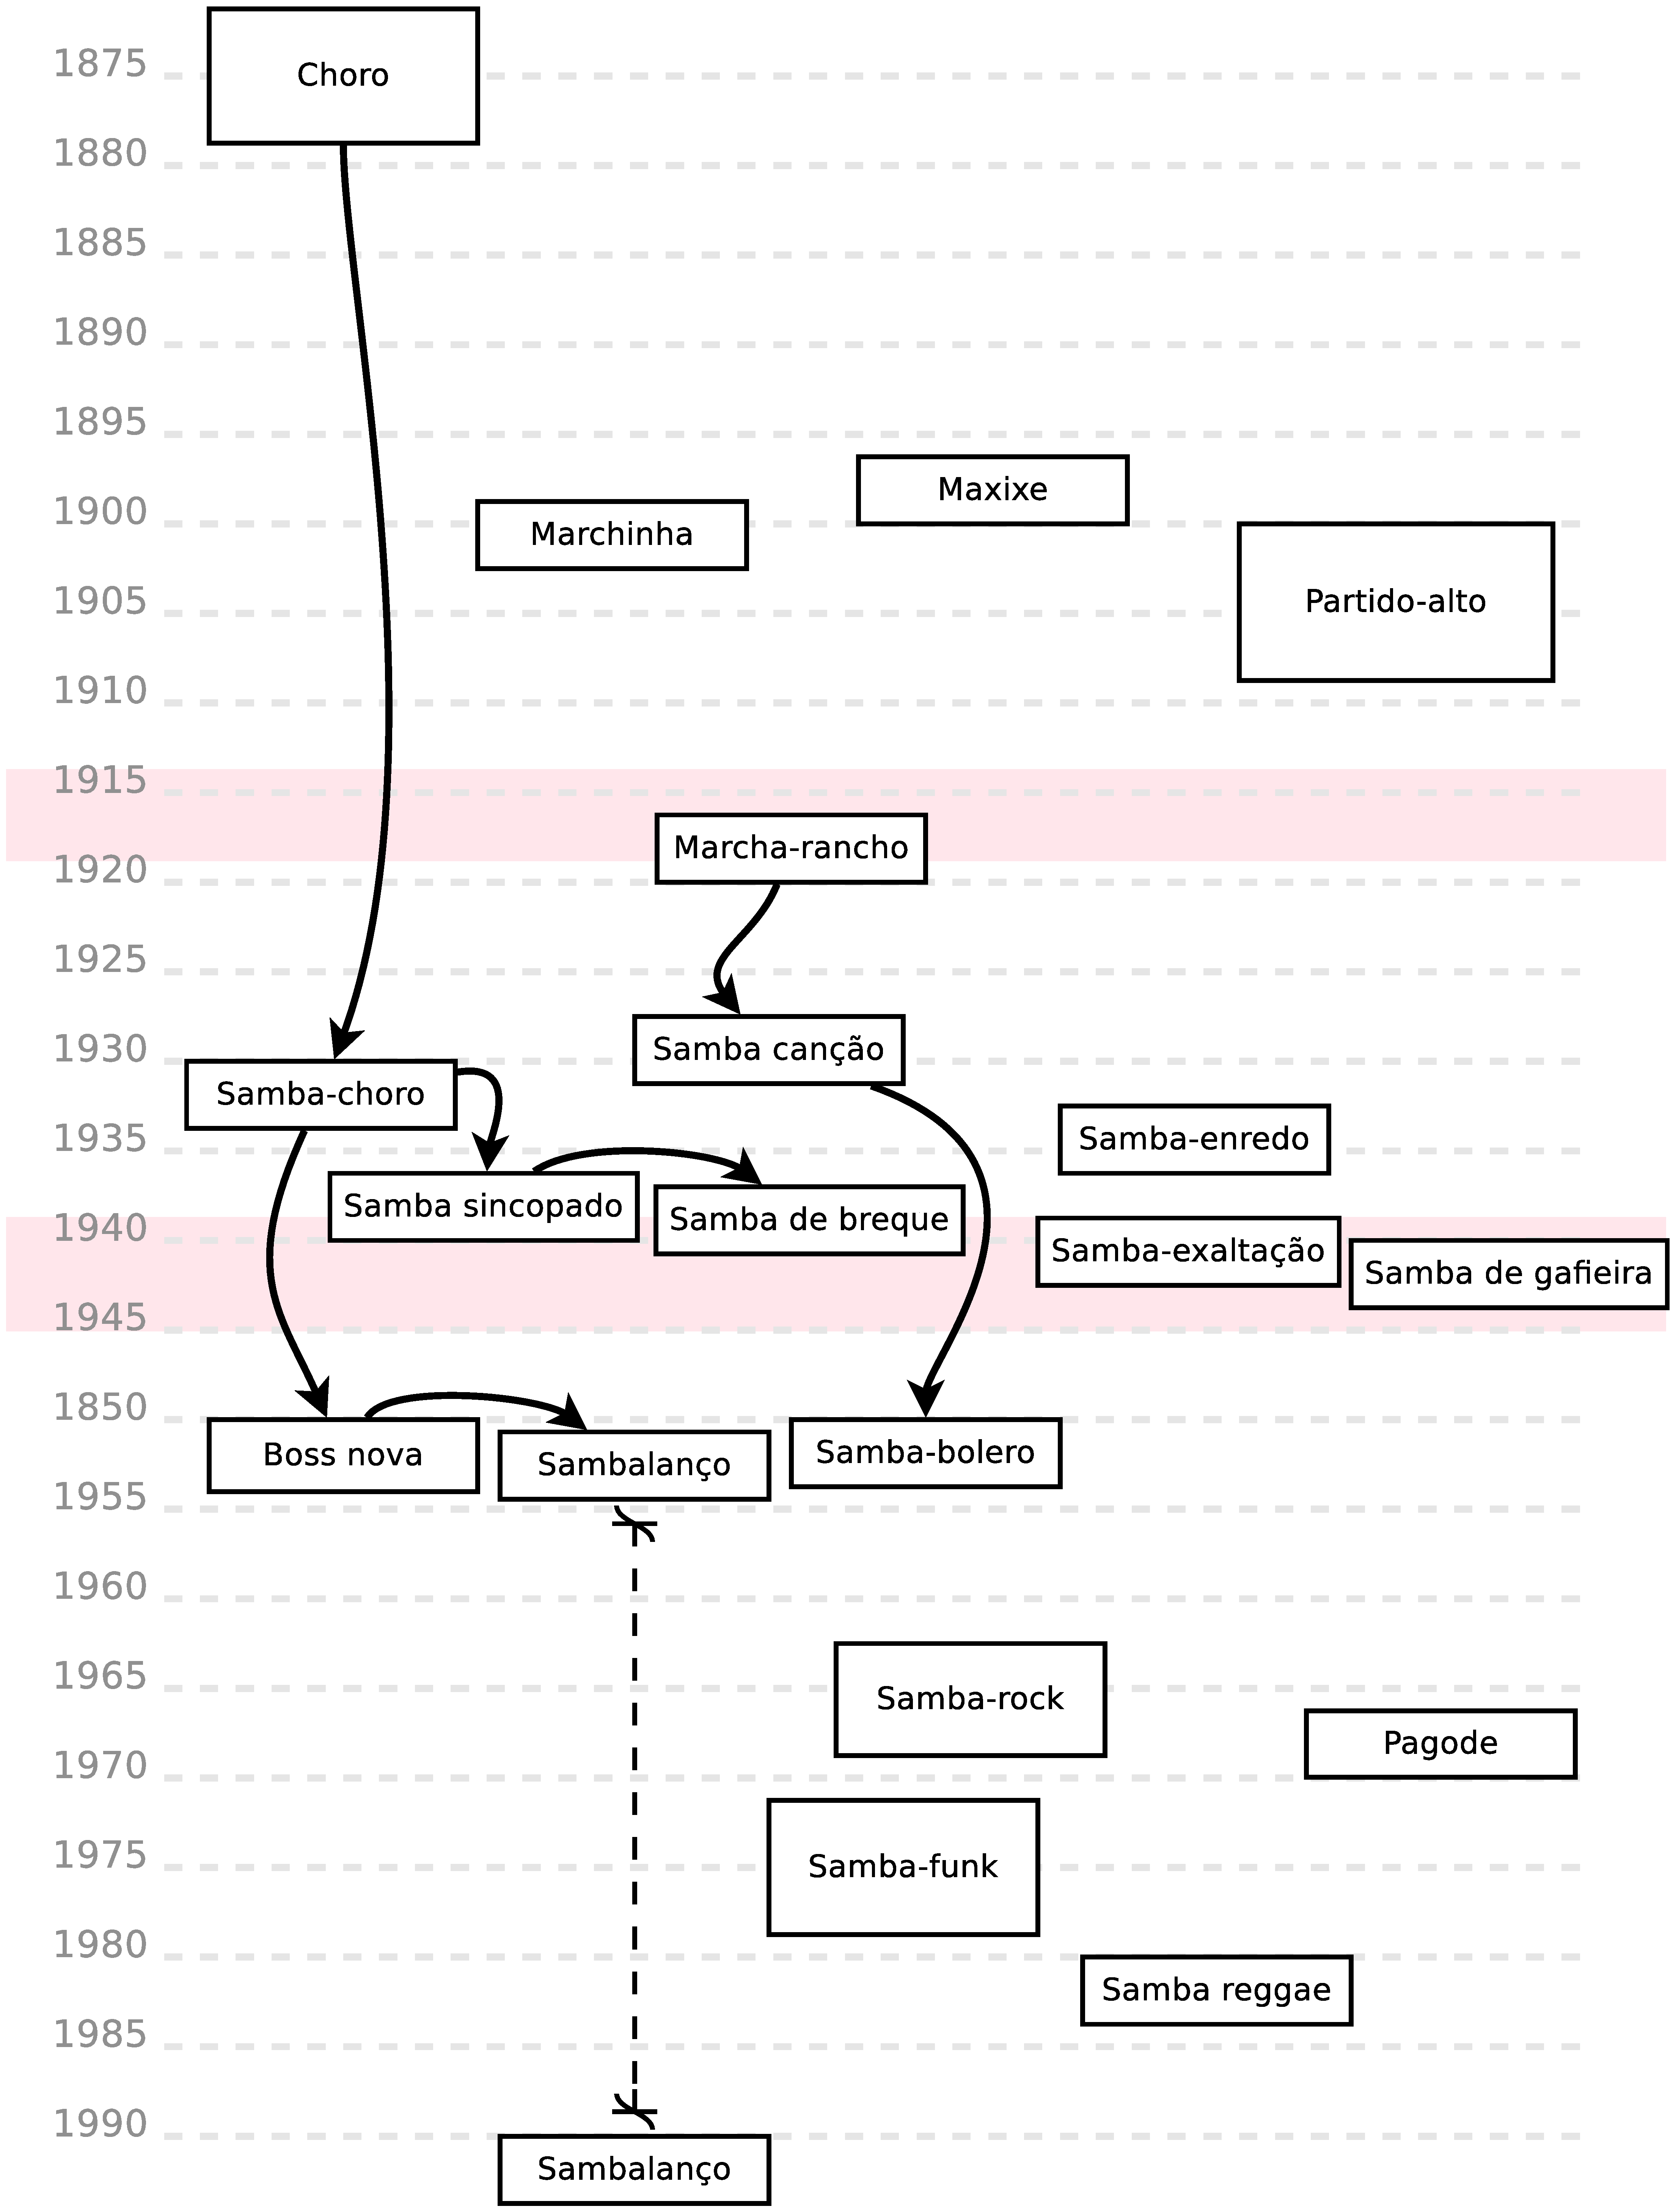
\includegraphics[width=1.0\textwidth]{chapters/cap-historia-musicasamba/musicatimeline.eps}
  \caption{Relação temporal entre os inícios dos subgêneros do samba.}
\label{fig:sambamusicatimeline1}
\end{figure}


